\section{Общие методы решения задач}
\subsection{Динамические модели}

Формирование эффективных уравнений динамики роботов, которые могут быть рассчитаны на ЭВМ за минимальное время, является одной из важнейших задач в робототехнике. Ее решение необходимо для моделирования динамики манипуляторов в масштабе реального времени, для разработки эффективных алгоритмов управления роботами с учетом динамики [2], для повышения эффективности исследования и разработки манипуляторов.

Одни из первых результатов в этой области принадлежат Kane [3] и Виттенбургу [4]. Полученные ими уравнения справедливы не только для роботов, но и для более широкого класса систем, состоящих из шарнирно связанных твердых тел. В дальнейшем было разработано большое количество алгоритмов формирования динамических уравнений манипуляторов, в которых использовались различные способы описания кинематики, расчета кинематических и динамических величин, а также различные формы уравнений динамики системы тел.

Описание кинематики – это способ задания систем координат, связанных со звеньями манипулятора, и выбора параметров, которые однозначно определяют взаимное положение звеньев и конфигурацию всего манипулятора. В представлении Денавита-Хартенберга [5] начала систем координат расположены в шарнирах, а их оси формируются по правилам, которые определяются кинематикой манипулятора. В другом методе описания кинематики локальные системы координат привязаны к центрам масс звеньев, а их оси направлены вдоль главных осей инерции. Параметры, определяемые относительно таких систем координат удобны для динамического анализа.

Еще одной характеристикой методов математического моделирования манипуляторов является способ расчета кинематических и динамических величин, определяющих математическую модель манипулятора. Для этого используются однородные координаты и матрицы преобразования координат размерности 4x4, определяющие относительное положение и ориентацию звеньев манипулятора [6]; матрицы поворотов размерности 3x3 и вектора относительных перемещений [6]; формулы Родриго [7]; ортогональные тензоры [8]; кватернионы; метод векторных параметров с использованием групп Ли .

Хотя вычислительная эффективность того или иного метода формирования динамических уравнений зависит в первую очередь от особенностей его реализации (использования рекурсивных преобразований, динамических аналогий и др.), можно отметить и существенную роль выбора подходящего способа расчета модели манипулятора. Например, матрицы преобразования однородных координат размерности 4x4, обладающие универсальностью в кинематическом описании, практически не используются в задачах реального времени из-за больших вычислительных затрат, необходимых для выполнения операций над ними. В то же время, использование матриц поворотов размера 3x3 позволяет получить эффективные алгоритмы расчета кинематики и динамики. 

Эффективно использование кватернионов, ортогональных тензоров, однако в ряде задач (например, при управлении в декартовых координатах) предпочтительнее использовать матричные представления.

Среди самых современных методов моделирования динамики манипуляторов можно отметить подходы, основанные на использовании нейронных  сетей [9], пространственных операторов [10], групп Ли, методов нечеткой логики [11]. Для описания динамики сложных структур (параллельных роботов, манипуляторов с большой избыточностью степеней подвижности, роботов-гуманоидов) используются методы расчета динамики в операционном пространстве роботов и другие.

\subsection{Уравнения движения}

Есть две основные формы записи уравнений движения [13]:

\begin{enumerate}
	\item уравнение в конфигурационном пространстве:
\begin{center}
	$M(q) \ddot q + C(q, \dot q)\dot q + G (q) = \tau$	
\end{center}
где $q, \dot q$ и $\ddot q$ -- положение, скорость и ускорение звена робота, $\tau$ -- силы/моменты приложенные к звену, $M(q)$ -- тензор инерции, $C(q, \dot q)$ -- матрица Кориолисовых и центробежных сил, $G(q)$ -- вектор гравитации;

	\item уравнение в операционном пространстве:
\begin{center}
	$\Lambda(x) \ddot x + \mu (x, \dot x) + \rho (x) = f$
\end{center}		
где $x$ -- положение схвата, $\dot x$ -- скорость схвата, $f$ -- действующие силы на схват, $\Lambda(x)$ -- матрица инерции в операционном пространстве, $\mu(x, \dot x)$ -- содержит Кориолисовы и центробежные составляющие, $\rho(x)$ -- вектор гравитации.

\end{enumerate}

Эти уравнения показывают функциональную зависимость: $H$ - функция от $q$, $\Lambda$ функция от $x$. Однако, эти зависимости часто отбрасывают, для более простого понимания. 

Строго говоря, коэффициенты уравнений зависят не только от $q, \dot q$ и $f_{ext}$, но также от динамической модели робототехнической системы.
Т.е. описание механизма отдельно для каждой из его частей: звенья, сочленения и их характеризующие их параметры. Динамическая модель состоит из:

\begin{itemize}
\item кинематической модели;
\item множества параметров инерции.
\end{itemize}

Для описание инерции твердого тела нужно десять параметров инерции: масса, расположение центра масс, шесть вращателльных параметров инерции. Однако, когда тела соединяют друг с другом их степени свободы ограничиваются и некоторые из этих параметров могут не оказывать влияния на поведение системы. Поэтому при составлении динамической модели робототехнического механизма от кинематической модели и измерения ее динамических характеристик, процедура сводится к идентификации значений множества основных параметров инерции, которые поддаются наблюдению в полученной системе.


\subsection{Алгоритмы основанные на уравнениях Лагранжа}

Существует четыре главных задачи динамики, которые решаются путем реализации описанных ниже алгоритмов. 
\begin{enumerate}
\item обратная задача динамики, когда требуется вычислить необходимые моменты/силы приводов звеньев для достижения заданной траектории (положение, скорость и ускорение);
\item прямая задача динамики, когда необходимо определить траекторию движения по заданным моментам/силам приводов звеньев;
\item определение матрицы инерции в конфигурационном пространстве;
\item определение матрицы инерции в операционном пространстве.
\end{enumerate}

Обратная задача решается для непосредственного управления роботом. Прямая -- для моделирования. Матрицы инерции находятся для анализа и управления.

Далее рассмотрены алгоритмы для решения этих задач. Сначала представлены алгоритмы основанные на уравнениях Эйлера-Лагранжа, после на методе Ньютона-Эйлера, Кейна и Аппеля [14].

\subsubsection{Алгоритм Uiker и Kahn}
Первая версия алгоритма была разработана в 1965 году J.J. Uicker и в основном использовалась для замкнутых кинематических цепей. В 1969 году M. Kahn доработал его таким образом, что стало возможным использовать его и для разомкнутых кинематических цепей. Также в алгоритм были внесены доработки в 1971 и 1981 годах, тогда N. Orleandea и T. Berea написали программную реализацию это метода в форме программного пакета для анализа динамики роботов. В дальнейшем различные модификации численных и символьных вычислений производили S.Mahil, M. Renaud, M. Tomas и Tesar, R. Waters, J. Hollerbach и многие другие.

Используя этот алгоритм можно решать как прямую, так и обратную задачи динамики. Также он позволяет вычислять матрицы динамической модели робота: матрицу инерции, матрицу Кориолисовых и центробежных сил и вектор гравитации. Уравнения динамики для робота с $n$ степенями свободы, соответствующие рассматриваемому алгоритму, представлены ниже.

\begin{align}\label{eq1}
P_i &= \sum_{j=i}^{n}
\left(
\sum_{k=1}^{j}
\left[
tr(\frac{\partial W_j}{\partial q_i} J_j \frac{\partial W_j^T}{\partial q_k})
\right] \ddot q_k 
\right.&\\
&+
\left.
\sum_{k=1}^{j} \sum_{l=1}^{j} 
\left[
tr(\frac{\partial W_j}{\partial q_i} J_j \frac{\partial^2 W_j^T}{\partial q_k \partial q_l})\dot q_k \dot q_l
\right]
-m_j \vec{q^T} \frac{\partial W_j}{\partial q_i} r_{jo}
\right)
\end{align}
где $P_i$ -- сила/момент привода, $W_i$ -- матрица трансформации от базовой к локальной системе координат $i$-ого звена, $J_i$ -- матрица инерции $i$-ого звена относительно локальной системы координат, $m_i$ -- масса звена $i$, $r_{j0}$ -- вектор от центра масс звена $i$ к началу базовой системы координат, выраженный в локальной системе координат звена $i$, $\vec g$ --вектор гравитации.

Матрица $W_i$ выражается, как:
\begin{equation}
W_i = A_1^0 A_2^1 ... A_i^{i-1}
\end{equation}
где $A_k^{k-1}$ -- матрица трансформации ($4 \times 4$) между системами координат $i$ и $i-1$.

	\begin{figure}[H]
	\center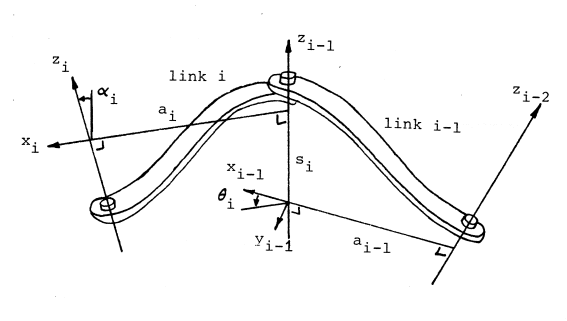
\includegraphics[width=0.8\linewidth]{1.png}
	\caption{Оси координат двух соседних звеньев}
	\label{fig:scr1}
	\end{figure}

Применение матриц однородных преобразований позволяет использовать одно уравнение и для призматических сочленений, и для вращательных. Системы координат в роботе выбираются в соответствии с конвенцией Денавита-Хартенберга. Таким образом, матрица трансформации из $i-1$ системы координат в $i$, представляет собой:
\begin{equation}
A_i^{i-1} = 
\begin{bmatrix}
1 & 0 & 0 & 0\\
a_i cos (q_i) & cos (q_i) & -sin (q_i) cos (a_i) & sin (q_i) sin (a_i)\\
a_i sin (q_i) & sin (q_i) & cos (q_i) cos (a_i) & -cos (q_i) sin (a_i)\\
s_i & 0 & sin (a_i) & cos (a_i)
\end{bmatrix}
\end{equation}

Оси локальной системы координат звена i представляются единичными векторами ($\vec x_i, \vec y_i, \vec z_i$). Эти системы координат зависят только от геометрических параметров системы, следовательно не совпадаются с главными осями инерции. Таким образом, вместо трех моментов инерции, получается тензор инерции. Uicker использовал тезор инерции $J_i$ размерности $4 \times 4$, который включает в себя и моментты инерции, и массы звеньев:


\begin{equation}
\begingroup\makeatletter\def\f@size{14}\check@mathfonts
J_i = 
\begin{bmatrix}
m_i & m_i x_{i0} & m_i y_{i0} & m_i z_{i0}\\
m_i x_{i0} & \frac{1}{2} (-I_{xx} + I_{yy} + I_{zz}) & I_{xy} & I_{xz}\\
m_i y_{i0} & I_{xy} & \frac{1}{2} (I_{xx} - I_{yy} + I_{zz}) & I_{yx} \\
m_i z_{i0} & I_{xz} & I_{yz} & \frac{1}{2} (I_{xx} + I_{yy} - I_{zz})
\end{bmatrix}
\endgroup
\end{equation}
где $x_{i0}, y_{i0}, z_{i0}$ -- координаты центра масс звена $i$ выраженные в базовой системе координат, $I_{xx}, I_{xy},...$ -- моменты инерции вокруг соответствующих осей.

Матрица инерции $J_i$ описывает распределение массы в звене $i$, а также зависит от положения центра масс относительно закрепленной системы координат.

Из матрицы трансформации $A_i^{i-1}$ мы видим, что ее частная производная относительно $q_i$ может быть определена аналитически. Тоже самое справедливо и для матрицы $W_i$. В этом случае нет рекурсивных отношений, поэтому метод Uicker принадлежит к классу нерекурсивных методов.

Теперь, когда мы выяснили общую структуру метода, детальнее рассмотрим как решаются прямая и обратная задачи динамики.

Обозначим $\dot q_i$ и $\ddot q_i$, как скорость и ускорение и запишем уравнение в следующей форме:
\begin{equation}\label{eq2}
P_i = \sum_{j=1}^{n}
H_{ij} (q) \ddot q_j
+
\sum_{k=1}^{n} \sum_{l=1}^{n}
C_{kl}^i (q) \dot q_k \dot q_l + g_i (q)
\end{equation}
где $H_{ij}, C_{kl}^i$ и $g_i$ -- скалярные функции зависящие от вектора обобщенных координат $q = [q_1,...,q_n]^T$. Что бы доказать это, заметим, что в соответствии с уравнением ~\ref{eq1}, эти функции зависят от частных производных матриц $W_i$. В свою очередь матрицы $W_i$ это функции обобщенных координат, из чего следует, что  частные производные матриц $W_i$ также зависят только от обобщенных координат. Теперь, представим модель ~\ref{eq2} в матричной форме:
\begin{equation}\label{eq3}
P = H(q) \ddot q + \dot q^T C(q) \dot q + g(q)
\end{equation}
где $P = [P_1,...,P_n]^T$ -- вектор управляющих сил/моментов, $H(q)$ -- матрица $n\times n$ инерции системы, $C(q)$ -- матрица Кориолисовых и центробежных сил, $g(q)$ -- $n$-вектор соответствующий действию гравитации на систему.

В модели ~\ref{eq3} $\dot q^T C(q) \dot q$ это $n$-вектор:
\begin{equation}
\dot q^T C(q) \dot q = 
\begin{bmatrix}
\dot q^T C^1(q) \dot q\\
\vdots\\
\dot q^T C^n(q) \dot q\\
\end{bmatrix}
\end{equation}
где $C^i(q)$ матрица $n \times n$, элементы которой соответствуют $C_{kl}^i (q)$ в уравнении \ref{eq2}. 

Итак, имея уравнение \ref{eq3} мы можем решить обратную задачу динамики, т.е. по заданным ($q, \dot q, \ddot q$) определить управляющие силы/моменты.

Чтобы решить прямую задачу, нужно определить $q(t)$ по известным моментам $P(t)$ для $t > t_0$ и начальными условиями $q(t_0)$ и $\dot q(t_0)$. Для это представим уравнение \ref{eq3} в следующей форме:
\begin{equation}
P = H(q) \ddot q + h(q, \dot q)
\end{equation}
где $h(q, \dot q) = \dot q^T C(q) \dot q + g(q)$.

Отсюда, выражая $\ddot q$ получим:
\begin{equation}
\ddot q = H(q)^{-1} (P - h(q, \dot q))
\end{equation}

$q(t)$ находится интегрированием полученного выражения.

Вычислительная сложность рассмотренного метода составляет $O(n^4)$. Такой алгоритм не подходит для расчета динамики современных роботов в реальном времени. Уравнение \ref{eq1} на 16-битном микропроцессоре вычисляется за 500 мс, для манипулятора с 3-мя степенями свободы и более 5 секунд для 6-степенного. Его можно несколько ускорить пренебрегая Кориолисовыми и центробежными скоростями на медленных режимах работы [14].

\subsubsection{Алгоритмы S. Mahil, S. Megahed и M. Renaud}
Эти алгоритмы представляют собой модификации Uicker-Kahn алгоритма, в которых авторы избавились от частной производной в уравнении и сократили количество арифметических операций.

В 1979 S.Mahil предложил заменить матрицы трансформации Денавита-Хертенберга формулой поворота Родрига. Чтобы описать суть этой формулы, представим вращение $i$ звена относительно $i-1$ на угол $q_i$. Введем вектор $\vec r_i$ прикрепленный к $i$ звену перед началом вращения. После вращения, в соответствии с формулой Родрига, этот вектор можно выразить, как:
\begin{equation}
\vec r_i = \vec r_i cos (q_i) + (1 - cos(q_i))(\vec e_i \times \vec r_i) \vec e_i + \vec e_i \times \vec r) sin (q_i)
\end{equation}
где $\vec e_i$ -- единичный вектор на оси прикрепленной к сочленению $i$.
 
Применим эту формулу для выражения матрицы трансформации $A_i^{i-1}$, которая описывает вращение $i$ системы координат относительно $i-1$. Заметим, что векторы $\vec q_{ij}, j=1,2,3$ -- единичные векторы осей $i$ системы. Тогда, матрица $A_i^{i-1}$:
\begin{equation}
A_i^{i-1} = 
\begin{bmatrix}
\vec q_{i1} & \vec q_{i2} & \vec q_{i3}
\end{bmatrix}
\end{equation}

Теперь, выразим вектор $\vec q_{ij}$, через формулу Родрига:
\begin{equation}
\vec q_{ij} = \vec q_{ij}^0 cos(q_i) + (1-cos(q_i)) (\vec e_{i} \times \vec q_{ij}^0) 
+ \vec e_{i} \times \vec q_{ij}^0 sin(q_i)
\end{equation}
где $\vec q_{ij}^0$ -- вектор оси $j$ $i$-ой системы координат перед вращением.

	\begin{figure}[H]
	\center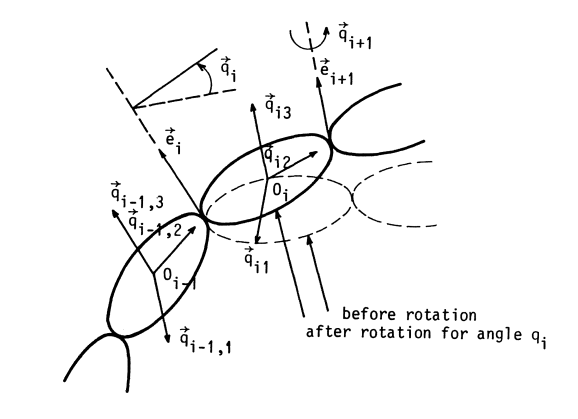
\includegraphics[width=0.8\linewidth]{2.png}
	\caption{Вращение звена $i$}
	\label{fig:scr2}
	\end{figure}

В отличие от кинематики Денавита-Хартенберга, формула Родрига применяется к локальным системам координат, которые прикреплены к звеньям в произвольных местах.
Наиболее удачным расположением обычно является центр масс звена, тогда системы координат вращения и инерции совпадают, что упрощает уравнение динамики, а также тензор инерции состоит только из главных моментов инерции звена.

В этом алгоритме фигурирует только два момента инерции -- продольный и поперечный.
Такое приближение возможно только для цилиндрических звеньев, длина которых много больше их диаметра. Это накладывает ограничения на применение этого алгоритма.

Алгоритм выводится из уравнения Лагранжа в матричной форме:
\begin{equation}\label{eq4}
P = \sum_{i=1}^{n} 
\left(
H^i (q) \ddot q + D^i (q, \dot q) \dot q + g^i (q)
\right)
\end{equation}
где $P$ -- вектор прикладываемых моментов/сил, $H^i (q), D^i (q, \dot q)$ -- $n \times n$ матрицы и $g^i (q)$ -- $n$-вектор.

Элементы матриц в уравнении \ref{eq4} могут быть выражены с использованием осей сочленений, локальных систем координат и векторов переноса, которые получаются применением формулы Родрига. Для вращательных сочленений:
\begin{align*}
H_{jk}^i = 
(Jn_i + m_i (\vec r_{ji} \times \vec r_{ki})) (\vec e_j \times \vec e_k)
&+ Js_i (\vec e_j \times \vec q_{i1}) (\vec e_k \times \vec q_{i1})
\\&- (\vec e_j  \times \vec q_{ki}) (\vec e_k \times \vec q_{ki})
\end{align*}
где $(j \le k \le i)$, $Jn_i$ -- поперечный момент инерции звена $i$, $Js_i$ -- продольный момент инерции звена $i$, $m_i$ -- масса звена $i$, $\vec r_{ij}$ -- вектор от $j$-ого сочленения к центру масс $i$-ого звена, в инерциальной системе.

Элементы матриц $D^i (q, \dot q)$ выражаются в следующей форме:
\begin{equation}
D_{kl}^i = 
\sum_{j=p+1}^{i}
\frac{\partial H_{kl}^i}{\partial q_j} \dot q_j - 
\frac{1}{2} \sum_{j=1}^{q}
\frac{\partial H_{jl}^i}{\partial q_k} \dot q_j
\end{equation}
где $p$ и $q$ зависят от $k$ и $l$. Это выражение включает частную производную от матриц и должны быть преобразованы к более простой для вычисления форме. Одно из уравнения, для вращательных сочленений:
\begin{align*}
\frac{\partial H_{kl}^i}{\partial q_j} &= 
(Jn_i + m_i \vec r_{ki} \times \vec r_{li})(\vec r_{k} \times \vec r_{j} \times \vec r_{l})+\\
& +m_i [\vec r_{k} \times \vec r_{j} (\vec R_{kj} \times \vec e_j \times r_{li})
- \vec e_l \times \vec r_{ki} (\vec R_{kj} \times \vec e_j \times \vec e_l) -\\
&- \vec e_k \times r_{li} (\vec R_{kj} \times \vec e_j \times \vec r_{li})] 
+ Js_i \vec e_l \times \vec q_{ik} (\vec e_k \times \vec e_j \vec q_{i1})
\end{align*}
где $\vec R_{kj}$ -- вектор от центра масс звена $j$ к центру масс звена $i$.

Выражение в матричной форме связывает элементы матриц Кориолисовых и центробежных сил с элементами матрицы инерции. Тем не менее, это выражение получается достаточно сложным. 

Этот алгоритм принадлежит к классу нерекурсивных, основанных на уравнениях Лагранжа. Сравнивая его с алгоритмом Uicker-Kahn, можно увидеть, что количество арифметических операций в этих алгоритмах имеют одинаковый порядок. Из этого следует, что его также практически невозможно реализовать для вычисления динамики в реальном времени. Тем не менее, основное достоинство этого алгоритма заключается в том, что он позволяется понять смысл динамических параметров в элементах матриц модели.

В 1981 году M. Renaud предложил эффективную процедуру вычисления параметром матриц частных производных, которые упоминались в алгоритме Uicker-Kahn. Алгоритм основывается на следующем свойстве матриц Денавита-Хартенберга [16]:
\begin{equation}\label{eq5}
\frac{\partial A_k^{k-1}}{\partial q_k} = Q A_k^{k-1}
\end{equation}
где, если звено вращательное:
\begin{equation}
Q = 
\begin{bmatrix}
0&0&0&0\\
0&0&-1&0\\
0&0&0&0\\
0&0&0&0\\
\end{bmatrix},
\end{equation} 
если звено призматическое:
\begin{equation}
Q = 
\begin{bmatrix}
0&0&0&0\\
0&0&0&0\\
0&0&0&0\\
1&0&0&0\\
\end{bmatrix}
\end{equation} 

Основываясь на отношении \ref{eq5}:
\begin{equation}
\frac{\partial W_j}{\partial q_i} = 
\begin{bmatrix}
0\\
\hline
\omega_i
\end{bmatrix}
W_j, (i \le j)
\end{equation}

\begin{equation}
\frac{\partial W_j}{\partial q_i \partial q_k} = 
\begin{bmatrix}
0\\
\hline
\omega_i
\end{bmatrix}
\begin{bmatrix}
0\\
\hline
\omega_k
\end{bmatrix}
W_j, (i \le k \le j)
\end{equation}
где $\omega_i$ -- матрица $3 \times 3$, элементы которой получены непосредственно из матрицы $W_j$.

Этот алгоритм также, принадлежит к классу нерекурсивных, основанных на уравнениях Лагранжа. Тем не менее, количество численных операций по прежнему очень велико, что делает невозможным его применение для расчета в режиме реального времени.

Также, стоит отметить, что в 1983 году M. Renaud предложил еще одну модификацию предыдущего алгоритма, вводя тензорное исчисление, а также ряд рекурсивных соотношений для вычисления динамической модели матриц. Но и эта модификация не привела к значительному сокращению числа операций. Однако, автор показал [17], что полученная аналитическая модель путем применения его процедур эффективна при вычислении. Но, к сожалению, порядок формирования модели не автоматизирован и должен осуществляться вручную. Это процедура достаточна сложна и не позволяет избежать ошибок. Таким образом, этот алгоритм также не может рассматриваться для вычислений в реальном времени.

\subsubsection{Алгоритм Vukobratovic-Potconjak}
В этом алгоритме, для описания расположения звеньев в пространстве, также как и предыдущем, используется формула Родрига. Такой подход облегчает динамический анализ механизмов, так как используются только главные моменты инерции.

Кинематическая часть этого алгоритма представляется выражениями:
\begin{equation}\label{eq7.1}
\omega_i = N(i) \dot q
\end{equation}
\begin{equation}\label{eq7.2}
\dot v_i = M(i) \dot q
\end{equation}
где $\omega_i$ -- вектор угловых скоростей звена $i$ выраженный в $i$-ой локальной системе координат, $v_i$ -- вектор линейных скоростей центра масс $i$-ого звена относительно $i$-ой локальной системы координат, $N(i), M(i)$ -- $3 \times n$ матрицы, зависящие от обобщенных координат, $\dot q$ -- $n \times 1$ вектор скоростей.

Подставляя уравнения \ref{eq7.1} и \ref{eq7.2} в кинетическую энергию системы, получим:

\begin{equation}
E_k = \sum_{i=1}^{n} (\frac{1}{2} m_i v_i^T v_i + \frac{1}{2} \omega_i^T J_i \omega_i)
\end{equation}

и, используя матричную форму представления уравнения Лагранжа:

\begin{equation}
\frac{d}{dt}
(\frac{\partial E_k}{\partial \dot q})
- \frac{\partial E_k}{\partial q} + \frac{E_p}{\partial q} = P
\end{equation}

получим динамическую модель робота:

\begin{equation}
P = H(q) \ddot q + h(q, \dot q)
\end{equation}

В выражении выше $m_i$ обозначает массу $i$ звена, $J_i$ -- диагональную матрицу $3 \times 3$ с главными моментами инерции, $E_k$ и $E_p$ -- кинетическую и потенциальную энергии всей системы, $P$ -- вектор управляющих моментов/сил.

Матрицы модели задаются следующими выражениями:
\begin{equation}
H(q) = \sum_{i=1}^{n}
(
m_i M(i)^T M(i) + N(i)^T J_i N(i)
)
\end{equation}
\begin{equation}
h(q, \dot q) = \frac{\partial (E_p - E_k)}{\partial q} + \dot H(q) \dot q
\end{equation}

Частные производные в последнем выражении это матрица инерции, $H(q)$, которая вычисляется из рекурсивных отношений, которые не представлены здесь по причине их внушительной сложности.

Количество арифметических операций в это алгоритме в несколько раз меньше, чем в алгоритме Uicker-Kahn. 

\subsubsection{Алгоритмы R. Waters и J. Hollerbach}
Эти алгоритмы разрабатывались для решения обратной задачи динамики, как частного случая алгоритма Uicker-Kahn.
Алгоритм не позволяет вычислять матрицу инерции системы, так как вторая производная обобщенных координат фигурирует в уравнении не явно. Именно поэтому эти алгоритмы не эквивалентны.

В соответствии с алгоритмом R. Waters, управляющие силы/моменты выражаются следующим уравнением:
\begin{equation}
\label{eq6}
P_i = 
\sum_{j=i}^{n}
\left[
tr(
\frac{\partial W_j}{\partial q_i} J_j \ddot W_j^T
)
- m_j \vec g^T \frac{\partial W_j}{\partial q_i} r_{i0}
\right]
\end{equation} 
со следующими рекурсивными отношениями:

\begin{equation}
W_j = W_{j-1} A_j^{j-1}
\end{equation}

\begin{equation}
\dot W_j = \dot W_{j-1} A_j^{j-1} + W_{j-1} \frac{\partial A_j^{j-1}}{\partial q_j} \dot q_j
\end{equation}

\begin{equation}
\ddot W_j = \ddot W_{j-1} A_j^{j-1} + 2 \dot W_{j-1}
\frac{\partial A_j^{j-1}}{\partial q_j} \dot q_j +
W_{j-1} \frac{\partial^2 A_j^{j-1}}{\partial q_j^2} \dot q_j^2 +
W_{j-1} \frac{\partial A_j^{j-1}}{\partial q_j} \ddot q_j  
\end{equation}

Эти рекурсивные соотношения уменьшают количество арифметических операций, требующихся на вычисление управляющих сил/моментов до $n^2$. Уменьшение количества операций по сравнению с алгоритмом Uicker-Kahn, связано с тем, что в рассматриваемом алгоритме матрица инерции системы не вычисляется явно, что не требует вычислять частные производные $\frac{\partial W_j}{\partial q_k \partial q_l}$. Однако, несмотря на внушительное уменьшение количество вычислений, этот алгоритм также не позволяет применять его для вычисления динамики в реальном времени.

Еще более значительное сокращение количества сложений и умножений в уравнении было предложено J. Hollerbach, который заметил, что частная производная $\frac{\partial W_j}{\partial q_i}$ может быть выражена как $(\frac{\partial W_j}{\partial q_i}) W_j^i$, где
\begin{equation}
W_j^i = A_{i+1}^{i} A_{i+2}^{i+1} ... A_{j-1}^j
\end{equation}
матрица трансформации из $i$-ой в $j$ локальную систему координат. Подставляя полученные выражения в уравнение \ref{eq6}, получим:
\begin{equation}
P_i = tr(\frac{\partial W_i}{\partial q_i}) D_i -
\vec{g}^T \frac{\partial W_i}{\partial q_i} c_i
\end{equation}
где 
\begin{equation}
D_i = J_i \ddot W_i^T + A_{i+1}^{i} D_{i+1},
\end{equation}
\begin{equation}
c_i = m_i r_{i0} + A_{i+1}^{i} c_{i+1}.
\end{equation}

Угловое ускорение $\ddot W_i^T$ вычисляется в прямой рекурсии от базы к схвату как и в алгоритме Waters. $D_i$ и $c_i$ вычисляются в обратной рекурсии от схвата к базе.

Таим образом, полученные соотношения позволяют достичь $30n-592$ операций умножения и $675n - 464$ операций сложения.

Несколько позже, Hollerbach еще более уменьшил количество операций применив вместо матриц трансформации $4 \times 4$ матрицы поворота $3 \times 3$ и векторы переноса. С этими изменениями количество операций, необходимых для вычисления моментов/сил стало: умножений 412n - 277, сложений 320n - 201.

% NEWTON
\subsection{Алгоритмы основанные на уравнениях Ньютона-Эйлера}

В этой части представлены алгоритмы основанные на уравнениях Ньютона-Эйлера. Их чаще используют для управления роботами.

Из уравнений Ньютона-Эйлера определяются силы/моменты действующие на звенья. Если принять за $F_i$ силу действующую на центр масс звена $i$, выраженную в локальной системе координат этого звена, а за $m_i$ массу $i$ звена, то второй закон Ньютона запишется, как:
\begin{equation}
F_i = m_i w_i
\end{equation}
где $w_i$ ускорение центра масс звена i. Уравнение Эйлера устанавливает взаимосвязь между моментами/силами и моментами инерции:
\begin{equation}
M_i = I_i \epsilon_i + \omega_i \times (I_i \omega_i)
\end{equation}
где $I_i$ -- матрица $3 \times 3$ с главными моментами инерции на диагонали,
$\epsilon_i$ -- угловое ускорение звена $i$, $\omega_i$ -- угловая скорость звена $i$.

Все векторы выражены в локальной системе координат $i$-ого звена, прикрепленной к центру масс. Оси локальной системы координат совпадают с осями инерции звена.

Выражая уравнения в неподвижной инерциальной системе координат уравнения имеют ту же форму, а матрица инерции находится по формуле: $J_i = A_i I_i A_i^T$. Матрица трансформации $A_i$ из локальной системы координат $i$-ого звена в зафиксированную систему. $J_i$ матрица инерции $i$ звена относительно базовой системы координат.

Далее рассмотрены алгоритмы Ньютона-Эйлера в неподвижной инерциальной и локальной системах координат.

\subsubsection{Алгоритм Vukobratovic-Stepanenko}

Уравнения динамики Ньютона-Эйлера впервые были применены к моделированию в 1973 году M. Vukobratovic и J. Stepanenko. Тогда была введена концепция рекурсивного решения прямой и обратной задач динамики. Этот алгоритм также упоминается как кинестатический, основанный на принципе Д'Аламбера. 

	\begin{figure}[H]
	\center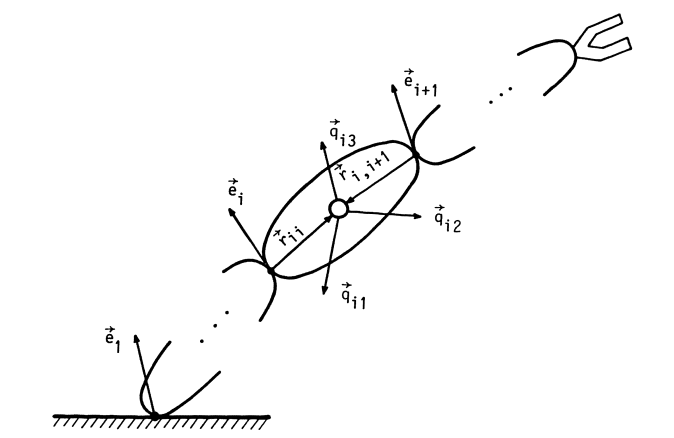
\includegraphics[width=0.8\linewidth]{3.png}
	\caption{Звено манипулятора}
	\label{fig:scr3}
	\end{figure}

На рисунке \ref{fig:scr3} представлено звено с необходимыми обозначениями для дальнейших выкладок. $\vec q_{ij}, (j=1,2,3)$ -- единичный вектор оси $j$ локальной системы координат звена $i$, $\vec r_{ii}$ -- вектор от $i$ сочленения до центра масс $i$ звена, $\vec r_{i, i+1}$ -- вектор от $i+1$ сочленения до центра масс $i$-ого звена, $\vec e_i$ -- единичный вектор $i$ сочленения, $i = 1,..., n$ 

Угловая скорость $\vec \omega_i$, угловое и линейное ускорения $\vec \epsilon_i, \vec w_i$ находятся из следующих уравнений:
\begin{equation}
\vec \omega_i = \vec \omega_{i-1} + \dot q_i \vec e_i
\end{equation}
\begin{equation}
\vec \epsilon_i = \sum_{j=1}^{i} \vec a_{ij} \ddot q_j + \vec a_i^0
\end{equation}
\begin{equation}
\vec w_i = \sum_{j=1}^{i} \vec \beta_i \ddot q_j + \vec \beta_i^0
\end{equation}
где коэффициенты $\vec a_{ij}, \vec a_i^0, \vec \beta_i^0$ получаются из соответствующих рекурсивных соотношений. Например $\vec a_i^0$:
\begin{equation}
\vec a_i^0 = \vec a_{i-1}^0 + \dot q_i \vec \omega_{i-1} \times \vec e_i
\end{equation}

Заметим два существенных свойства объединяющие эти отношения:
\begin{enumerate}
\item свойства рекурсивности;
\item ускорения $\ddot q_i$ в обоих уравнениях, что позволяет находить матрицы инерции и решать прямую задачу динамики.
\end{enumerate}

Инерционная сила и момент могут быть выражены, как:
\begin{equation}
\vec F_i = \sum_{j=1}^{i}
\vec a_{ij} \ddot q_j + \vec a_i^0
\end{equation}
\begin{equation}
\vec M_i = \sum_{j=1}^{i}
\vec b_{ij} \ddot q_j + \vec b_i^0
\end{equation}
где $b_{ij}$ и $b_{i}^0$ получаются из уравнений динамики Эйлера и выражают только моменты инерции, но не тензор инерции. Уравнение движения в матричной форме:
\begin{equation}
P = H(q) \ddot q  + h(q, \dot q)
\end{equation}
где $H(q)$ -- матрица инерции $n \times n$:
\begin{equation}
H_{ik} = - \vec e_i \sum_{j=max(i,k)}^{n}
(\vec b_{jk} + \vec r_{ji} \times \vec a_{jk}), (i,k=1,...,n)
\end{equation}
и $h(q, \dot q)$ вектор с $n$ элементами:
\begin{equation}
h_i = - \vec e_i \sum_{j=1}^{n} (
\vec r_{ji} \times (\vec a_k^0 + \vec G_j) + \vec b_j^0
)
\end{equation} 
где $\vec G_j$ вектор гравитации, действующий на звено $j$. Все уравнения записаны для вращательных звеньев, но могут быть легко приведены к форме для призматических путем обнуления тех членов уравнений, которые представляют угловые скорости и ускорения.

Для рассмотренного алгоритма, количество умножений равно $\frac{3}{4} n^3 + 28 n^2 + \frac{525}{2} n$, а для операций сложения $\frac{4}{3} n^3 + 20 n^2 + \frac{530}{2} n$.

Для решения только обратной задачи кинематики этот алгоритм можно представить в несколько иной форме. Тогда, кинематика представляется следующими тремя рекурсивными выражениями:
\begin{equation}
\omega_i = \omega_{i-1} + \dot q_i e_i,
\end{equation}
\begin{equation}
\epsilon = \epsilon_{i-1} + \ddot q_i e_i + \dot q_i (\omega_{i-1} \times e_i),
\end{equation}
\begin{align*}
w_i &= w_{i-1} - \epsilon_{i-1} \times r_{i-1, i} + \epsilon_i \times r_{ii} - \omega_{i-1} \times (\omega_{i-1} \times r_{i-1,i})\\
&+ \omega_i \times (\omega_i \times r_{ii})
\end{align*}
а динамика уравнениями Ньютона-Эйлера:
\begin{equation}
F_i = m_i w_i
\end{equation}
\begin{equation}
M_i = J_i \epsilon_i + \omega_i \times (J_i \omega_i)
\end{equation}
где $J_i = A_i I_i A_i^T$ матрица $3 \times 3$ инерции звена $i$ относительно базовой системы координат.

Обозначив $R_i$ и $M_i$ силу и момент, с которыми звено $i$ действует на звено $i-1$, получим следующие рекурсивные отношения.

\begin{equation}
R_i = R_{i+1} - F_i - G_i
\end{equation}

\begin{equation}
M_i = M_{i+1} + (r_{ii} - r_{i,i+1}) \times R_{i+1} + r_{ii} \times (F_i + G_i) - M_i
\end{equation}

где $R_{n+1}, M_{n+1}$ сила и момент действующие на $n$-ое звено (схват). Эти соотношения вычисляются в обратной рекурсии от схвата к базе $i = n,...,1$. 

Управляющие моменты вычисляются, как:
\begin{equation}
P_i = M_i e_i
\end{equation}
а силы, для призматических звеньев:
\begin{equation}
F_i = R_i e_i
\end{equation}

Количество операций умножения и сложения равны $225n$ и $152n$, соответственно.

Также этот алгоритм был усовершенствован J. Luh и M. Walker, для чего все кинематические и динамические переменные были выражены в локальных системах координат звеньев. Это привело к еще большему сокращению численных операций для вычисления динамики: $150n - 48$ умножений и $131n - 48$ сложений.

Необходимо отметить, что этот алгоритм решает только обратную задачу динамики.

Одним из основных достоинств этого алгоритма является простота описания сложных сочленений, имеющих 6-ть степеней свободы. Однако это достоинство одновременно является и недостатков, так как усложняет реализацию алгоритма по отношению к простым механизмам. 

Что касается количества арифметических операций, то их значительно больше, по сравнению с описанных ранее рекурсивными алгоритмами основанными на уравнениях Ньютона-Эйлера, так как алгоритм нерекурсивный.

\subsection{Алгоритмы основанные на уравнениях Аппеля}
Уравнения Аппеля основаны на функции Гиббса "энергии ускорения". Кинематика описана таким же образом как и в алгоритмах на базе Ньютона-Эйлера.

Относительное расположение соседних двух звеньев описывается формулой Родрига. Матрицы трансформации $A_i^{i-1}$ между системами координат звена $i-1$ и локальной системы координат звена $i$ получается таким же способом, как и в методе Ньютона-Эйлера. Отношения для кинетических параметров, также аналогичны:

\begin{equation}
\omega_i = A_i^{i-1} \omega_{i-1} + \dot q_i e_i
\end{equation} 
\begin{equation}
\epsilon_i = A_i^{i-1} \epsilon_{i-1} + \ddot q_i e_i + \dot q_i (\omega_i \times e_i)
\end{equation}
\begin{align*}
w_i = A_i^{i-1} (w_{i-1} - \epsilon_{i-1} \times r_{i-1,i} &- \omega_{i-1} \times (\omega_{i-1} \times r_{i-1,i})) + \\
&+ \epsilon_i \times r_{ii} + \omega_i \times (\omega_i \times r_{ii})
\end{align*}
где $e_i$ -- единичный вектор на оси $i$-ого сочленения выраженный в локальной системе координат звена $i$, $r_{ij}$ -- вектор от сочленения $j$ до центра масс звена $i$, выраженный в локальной системе координат звена $i$.

Динамика механизма описывается уравнениями Гиббса-Аппеля:
\begin{equation}
\frac{\partial G}{\partial \ddot q_i} = Q_i, (i=1,...,n)
\end{equation}
где $G$ -- функция "энергии ускорения", $Q_i$ -- обобщенная сила.

Функция "энергии ускорения" может быть выражена как сумма:
\begin{equation}
G = \sum_{i=1}^n G_i
\end{equation}
где $G_i$ -- функция Гиббса для звена $i$, которая, в свою очередь, определется из выражения:
\begin{equation}
G_i = \frac{1}{2} m_i w_i^2 + \frac{1}{2} \epsilon_i^T J_i \epsilon_i + 2 (\omega_i \times J_i \omega_i) \epsilon_i
\end{equation}

Подставляя в последнее выражения рекурсивные отношения для кинематики робота, получаем динамическую модель робота в форме:

\begin{equation} \label{eq8}
H(q) \ddot q + h_c (q, \dot q) = Q
\end{equation}
где $Q = [Q_1,...,Q_n]$ -- вектор обобщенных сил. Вектор обобщенных сил это разница, между управляющими силами/моментами и вектором описывающим действие гравитации на систему $g(q)$:
\begin{equation}
Q = P - g(q)
\end{equation}

Подставляя полученное уравнение в уравнение \ref{eq8}, получим:
\begin{equation}
H(q) \ddot q + h (q, \dot q) = P
\end{equation}
где $h (q, \dot q) = h_c (q, \dot q) + g(p)$.

Этот алгоритм позволяет решать как прямую, так и обратную задачи динамики. Вычислительная сложность: $\frac{7}{3} n^3 + 27 n^2 + \frac{722}{3} n + 9$ -- умножений, $\frac{10}{3} n^3 + \frac{43}{2} n^2 + \frac{931}{6} n + 6$ -- сложений.


\subsection{Алгоритмы основанные на уравнениях Кейна}
Алгоритм основывается на динамических уравнениях Kane. Эти уравнения выражаются из основных теорем механики. Алгоритм Kane напрямую зависит от динамических уравнения Ньютона-Эйлера. Динамические уравнения Kane не ограничиваются лишь робототехническими системами, но также применяются и к более широкому классу механизмов, в том числе, например, они используются в космических аппаратах с несколькими соединенными твердыми телами.

Считается, что робот состоит из $n$ соединеных твердых тел, каждое из которых имеет по 6 степеней свободы. Относительная ориентация соседних звеньев описывается следующими четырьмя параметрами Эйлера:

\begin{align*}
\epsilon_{il} &= e_{il} sin (\frac{q_i}{2}), (l=1,2,3)\\
\epsilon_{i4} &= e_{i4} cos (\frac{q_i}{2}). 
\end{align*}

где $e_i = (e_{i1}, e_{i2}, e_{i3})$ -- единичный вектор на оси, вокруг которой $i-1$ локальная система координат переходит в $i$ в результате вращения, $q_i$ -- угол, $e_{i4} = 1$. Можно показать, что параметры Эйлера эквивалентны формеле Родрига, когда сочленения с одной степенью свободы связаны. 

\begin{equation}
r' = r + 2 sin (\frac{q_i}{2}) e_i \times (e_i \times r) + 2 sin (\frac{q_i}{2}) cos (\frac{q_i}{2}) (e_i \times r)
\end{equation}
где $r$ -- вектор до вращения, $r'$ -- вектор после вращения на угол $q_i$ вокруг оси $e_i$. Сделав замену $\epsilon_i =e_i sin (\frac{q_i}{2}) $ и $\epsilon_{i4} = cos  (\frac{q_i}{2})$, получим:
\begin{equation}
r' = r + 2 \epsilon_i \times (\epsilon_i \times r) + 2 sin (\frac{q_i}{2}) \epsilon_{i4} (\epsilon_i \times r)
\end{equation}

Кинематические соотношения в этом алгоритме состоят из  выражения для скоростей и ускорений звеньев в терминах параметров Эйлера:

\begin{equation}
\omega_i = \sum_{k=1}^{i} \omega'_i
\end{equation}
где $\omega_i$ -- угловая скорость звена $i$ относительно базовой системы координат, $\omega'_k$ -- относительная угловая скорость звена $k$ относительно звена $k-1$. Это соотношение можно переписать в рекурсивной форме:

\begin{equation}
\omega_i = \omega_{i-1} + \omega'_i
\end{equation}

Несложно заметить, что это уравнение совпадает с ранее рассмотренным. Таким образом, единственное различие заключается в том, что для вычисления кинематических и динамических параметров уравнений используется нерекурсивные соотношения.

\subsection{Эффективность алгоритмов}

В таблице ~\ref{alhgorithms} представлены результаты анализа методов описания динамики манипуляторов по форме уравнений, вычислительной эффективности (для манипуляторов с шестью степенями свободы); также отражено, обеспечивает ли данный алгоритм замкнутость уравнений и возможность решения прямой задачи динамики.

Как показывает анализ таблицы, многие эффективные в вычислительном плане методы не обеспечивают замкнутости системы уравнений динамики, что ограничивает их применение в задачах управления, а также при анализе влияния различных динамических коэффициентов на движение манипулятора.

В последние годы для повышения эффективности уравнений динамики широко применяются символьные преобразования и алгоритмы распараллеливания вычислений. Применение символьных преобразований, способствует уравниванию различных алгоритмов по вычислительной эффективности. Поэтому важными критериями оценки алгоритма становятся  хорошая  алгоритмизуемость (удобство программирования), замкнутость уравнений, возможность применения символьных преобразований и алгоритмов распараллеливания.

Кроме того, можно отметить, что в работах ряда авторов указывается, что во многих случаях (например в задачах управления роботами) наиболее подходящим способом описания динамики являются уравнения Лагранжа. Это отмечено и в работе [18], где утверждается, что при реализации динамических алгоритмов на параллельных процессорах зависимость данных в методах, основанных на уравнениях Ньютона-Эйлера, намного сильнее, чем при использовании уравнений Лагранжа.

% Please add the following required packages to your document preamble:
% \usepackage{multirow}
% \usepackage{graphicx}
% \usepackage[normalem]{ulem}
% \useunder{\uline}{\ul}{}
\begin{table}[H]
\centering
\caption{Алгоритмы}
\label{alhgorithms}% Please add the following required packages to your document preamble:
\begin{tabular}{|l|l|r|r|c|c|}
\hline
\multicolumn{1}{|c|}{\multirow{2}{*}{\begin{tabular}[c]{@{}c@{}}Форма\\ уравнений\end{tabular}}} & \multicolumn{1}{c|}{\multirow{2}{*}{\begin{tabular}[c]{@{}c@{}}Авторы\\ алгоритма\end{tabular}}} & \multicolumn{2}{c|}{Число операций} & \multirow{2}{*}{\begin{tabular}[c]{@{}c@{}}Замкнутость\\ уравнений\end{tabular}} & \multirow{2}{*}{\begin{tabular}[c]{@{}c@{}}Прямая\\ задача\end{tabular}} \\ \cline{3-4}
\multicolumn{1}{|c|}{} & \multicolumn{1}{c|}{} & \multicolumn{1}{c|}{*} & \multicolumn{1}{c|}{+} &  &  \\ \hline
\multirow{5}{*}{Лагранж} & Uicker/Kahn & 66271 & 51548 & + & + \\ \cline{2-6} 
 & \begin{tabular}[c]{@{}l@{}}Vukobratovic/\\ Potconjak\end{tabular} & 37189 & 5652 & - & + \\ \cline{2-6} 
 & Hollerbach 3x3 & 2195 & 1719 & - & - \\ \cline{2-6} 
 & Renaud & 992 & 776 & - & + \\ \cline{2-6} 
 & Li & 951 & 842 & - & + \\ \hline
\multicolumn{1}{|c|}{\multirow{5}{*}{Ньютон-Эйлер}} & \begin{tabular}[c]{@{}l@{}}Vukobratovic/\\ Stepanenko\end{tabular} & 2907 & 2068 & + & + \\ \cline{2-6} 
\multicolumn{1}{|c|}{} & Walker/Orin & 1771 & 1345 & - & + \\ \cline{2-6} 
\multicolumn{1}{|c|}{} & Wang/Ravani & 1659 & 1252 & - & + \\ \cline{2-6} 
\multicolumn{1}{|c|}{} & \begin{tabular}[c]{@{}l@{}}Luh/Walker/\\ Paul\end{tabular} & 792 & 662 & - & - \\ \cline{2-6} 
\multicolumn{1}{|c|}{} & \begin{tabular}[c]{@{}l@{}}Balafoutis/\\ Patel/Misra\end{tabular} & 489 & 420 & - & - \\ \hline
Д'Аламбер & Lee/Nigam & 2963 & 2209 & + & + \\ \hline
Аппель & Попов & 2929 & 2500 & + & + \\ \hline
Кейн & Ma/Xu & 1020 & 851 & - & - \\ \hline
\end{tabular}
\end{table}

\section{Работы по алгоритмам}

При выводе уравнений динамики манипуляторов используются различные законы и формулировки общих уравнений динамики систем. Среди них можно выделить методы, основанные на уравнениях Лагранжа, Ньютона-Эйлера, Д'Аламбера, Гаусса, Аппеля, Кейна.

Уравнения динамики в форме Лагранжа впервые были получены в работе Uicker [19] и получили дальнейшее развитие в плане повышения эффективности в работах Kahn, Vukobratovic, Mahil, Renaud, Thomas и Tesar. Все перечисленные методы позволяли решать прямую и обратную задачу динамики, были удобны в алгоритмической реализации (кроме Renaud), но обладали низкой вычислительной эффективностью. Waters и Hollerbach [6] применили рекурсивные преобразования при выводе динамических уравнений, причем при использовании матриц поворотов $3 \times 3$ было получено значительное сокращение числа операций, но эти методы позволяли решать лишь обратную задачу динамики, поэтому не были пригодны для моделирования. Рекурсивные преобразования и формулы Родриго использовали Vukobratovic и Potkonjak, причем их метод позволял решать и прямую задачу динамики, хотя его вычислительная эффективность и не столь высока. Значительный прогресс в сокращении числа операций достигнут в работах Renaud и Li, также применивших рекурсивные соотношения.

Среди методов, использующих уравнения Ньютона-Эйлера и позволяющих решать прямую задачу динамики, можно отметить работы Vukobratovic и Stepanenko, Orin и Walker, Armstrong, Wang и Ravani. Во всех работах применяется рекурсия. Отметим также алгоритм Balafoutis [8], в котором за минимальное число операций решена обратная задача динамики.

Использование принципа Д'Аламбера для уравнений Лагранжа позволяет получить достаточно эффективные динамические соотношения, в которых в явном виде отражены эффекты влияния вращательного и поступательного движения звеньев на динамику манипулятора. В работе Попова получены уравнения динамики в явном виде с использованием уравнений Аппеля, позволяющие решать прямую и обратную задачи динамики. Уравнения Кейна особенно эффективны для расчета обобщенных моментов манипуляторов с замкнутыми кинематическими цепями. В работах Коноплева для описания динамики манипуляционных систем применяются агрегативные модели; метод удобен для применения символьных преобразований. Погореловым разработан пакет программ моделирования динамики широкого класса механических систем, включая роботы-манипуляторы. Интересный подход и язык программирования уравнений движения сложных механических систем, состоящих их твердых тел, предложен Сазоновым.

Полный анализ основных достижений в области моделирования динамики роботов, начиная с первых работ 60-70 годов прошлого века по 2000 гг., дан в работе Featherstone и Orin [12].

